\hypertarget{phonefirewall__administration_8c}{
\section{phonefirewall\_\-administration.c File Reference}
\label{phonefirewall__administration_8c}\index{phonefirewall\_\-administration.c@{phonefirewall\_\-administration.c}}
}
{\tt \#include $<$stdio.h$>$}\par
{\tt \#include $<$stdlib.h$>$}\par
{\tt \#include $<$errno.h$>$}\par
{\tt \#include $<$string.h$>$}\par
{\tt \#include $<$sqlite3.h$>$}\par
{\tt \#include \char`\"{}libphonefirewall.h\char`\"{}}\par
{\tt \#include \char`\"{}logfile.h\char`\"{}}\par


Include dependency graph for phonefirewall\_\-administration.c:\nopagebreak
\begin{figure}[H]
\begin{center}
\leavevmode
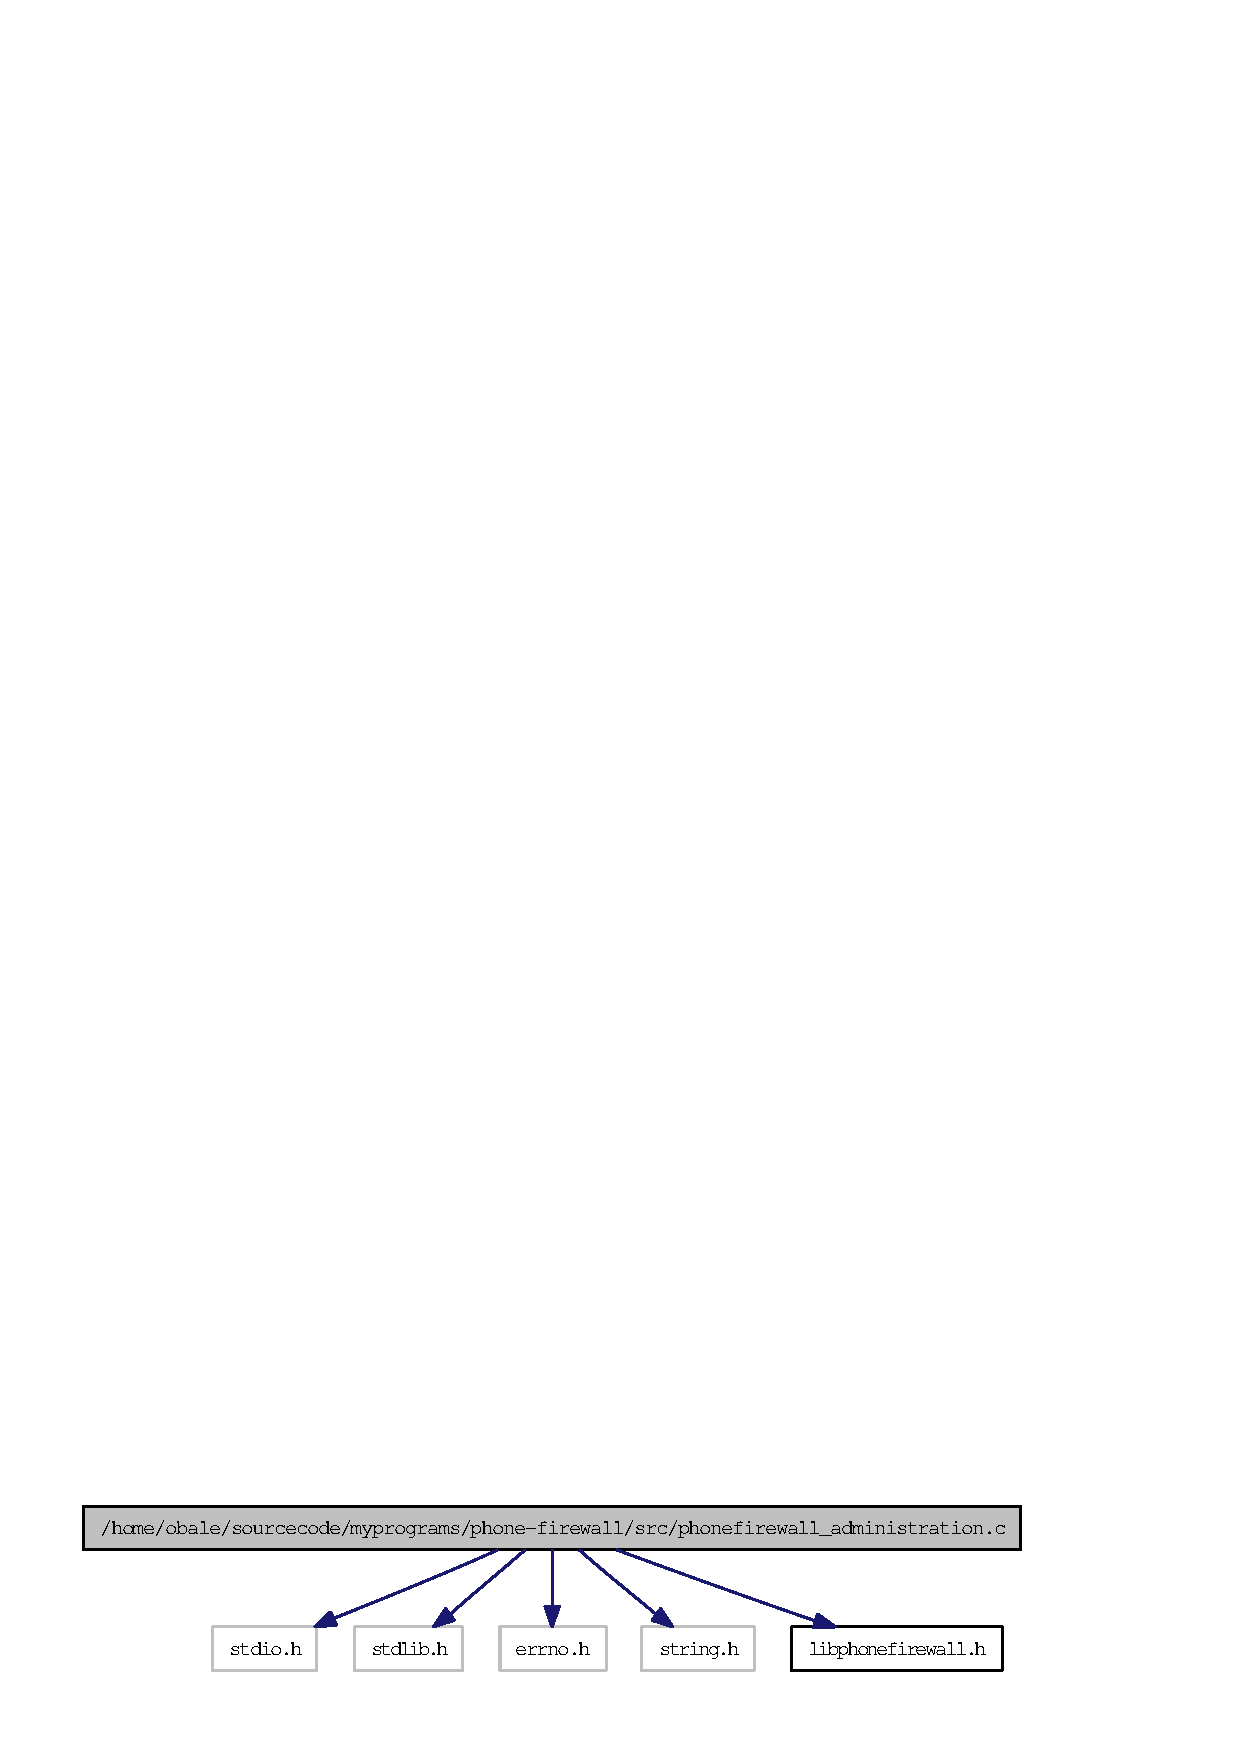
\includegraphics[width=285pt]{phonefirewall__administration_8c__incl}
\end{center}
\end{figure}
\subsection*{Functions}
\begin{CompactItemize}
\item 
int \hyperlink{phonefirewall__administration_8c_f306b60195d745190ef3e30e7d0a107e}{evaluate\_\-stmt} (sqlite3\_\-stmt $\ast$pp\_\-stmt, struct \hyperlink{structEntry}{Entry} $\ast$p\_\-entry)
\item 
int \hyperlink{phonefirewall__administration_8c_36847ed3459e2a89038772ece42a017d}{add\_\-blacklist\_\-entry} (int country\_\-code, int area\_\-code, unsigned long long number, char $\ast$name, char $\ast$reason, int priority)
\item 
int \hyperlink{phonefirewall__administration_8c_eec16cb88eb546b1a2490e6716d75f8b}{add\_\-whitelist\_\-entry} (int country\_\-code, int area\_\-code, unsigned long long number, char $\ast$name, char $\ast$reason, int priority)
\item 
int \hyperlink{phonefirewall__administration_8c_4eee00c845ad4a60eaccef8c41151ea4}{rm\_\-blacklist\_\-entry} (int country\_\-code, int area\_\-code, unsigned long long number)
\item 
int \hyperlink{phonefirewall__administration_8c_307d220ee8e63926af279460532787ff}{rm\_\-whitelist\_\-entry} (int country\_\-code, int area\_\-code, unsigned long long number)
\item 
int \hyperlink{phonefirewall__administration_8c_f28c4b8fd3fdfe5e70df391cf40ca9f2}{check\_\-blacklist\_\-entry} (int country\_\-code, int area\_\-code, unsigned long long number, int priority)
\item 
int \hyperlink{phonefirewall__administration_8c_f144fe0aa2eb227fe646da21048388a5}{check\_\-whitelist\_\-entry} (int country\_\-code, int area\_\-code, unsigned long long number, int priority)
\end{CompactItemize}


\subsection{Function Documentation}
\hypertarget{phonefirewall__administration_8c_36847ed3459e2a89038772ece42a017d}{
\index{phonefirewall\_\-administration.c@{phonefirewall\_\-administration.c}!add\_\-blacklist\_\-entry@{add\_\-blacklist\_\-entry}}
\index{add\_\-blacklist\_\-entry@{add\_\-blacklist\_\-entry}!phonefirewall_administration.c@{phonefirewall\_\-administration.c}}
\subsubsection{\setlength{\rightskip}{0pt plus 5cm}int add\_\-blacklist\_\-entry (int {\em country\_\-code}, int {\em area\_\-code}, unsigned long long {\em number}, char $\ast$ {\em name}, char $\ast$ {\em reason}, int {\em priority})}}
\label{phonefirewall__administration_8c_36847ed3459e2a89038772ece42a017d}


Add a number to the blacklist. The number will be blocked after that.

\begin{Desc}
\item[Parameters:]
\begin{description}
\item[{\em country\_\-code}]The country code (for example 39 for Italy, 43 for Austria, and so one) \item[{\em area\_\-code}]The area code which indicates your mobile operator. \item[{\em number}]The telephone number of the person (without country and area code. \item[{\em name}]The name of the person. \item[{\em reason}]Why you have blocked this person. \item[{\em priority}]Gives the \hyperlink{structentry}{entry} a priority. 0 is standard. If the priority is higher the value will be also blocked/accepted if a higher priority is choosen. \par
 The value \char`\"{}PRIO\_\-ALL\char`\"{} stands for all priorities.\end{description}
\end{Desc}
\begin{Desc}
\item[Returns:]If all goes well 0 (zero) otherwise an errno code. \end{Desc}


Definition at line 74 of file phonefirewall\_\-administration.c.

References DB\_\-FILE, ERR\_\-FLAG, MAX\_\-LINE\_\-LENGTH, PRIO\_\-ALL, STMT\_\-SIZE, TB\_\-AREACODE, TB\_\-COUNTRYCODE, TB\_\-NAME, TB\_\-NUMBER, TB\_\-PRIORITY, TB\_\-REASON, and write\_\-logentry().

Here is the call graph for this function:\nopagebreak
\begin{figure}[H]
\begin{center}
\leavevmode
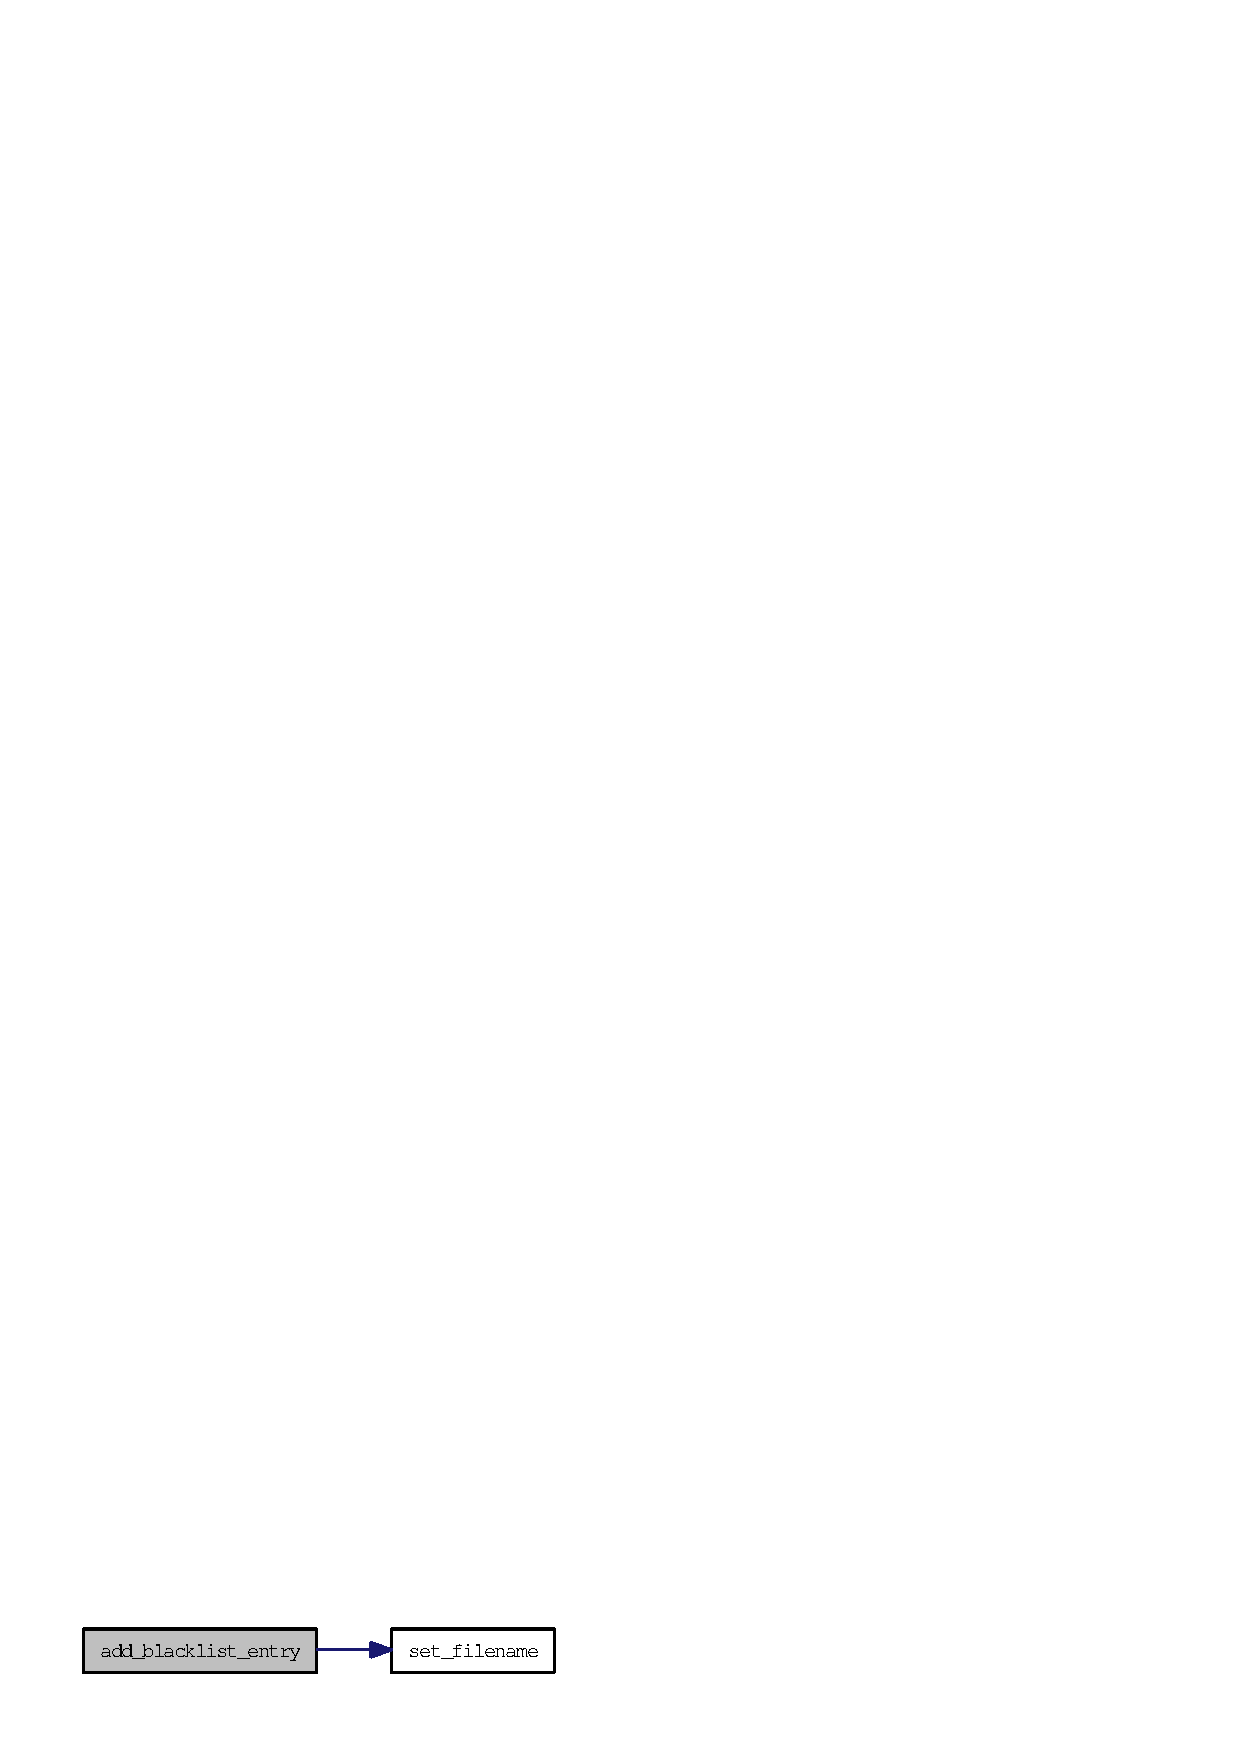
\includegraphics[width=185pt]{phonefirewall__administration_8c_36847ed3459e2a89038772ece42a017d_cgraph}
\end{center}
\end{figure}
\hypertarget{phonefirewall__administration_8c_eec16cb88eb546b1a2490e6716d75f8b}{
\index{phonefirewall\_\-administration.c@{phonefirewall\_\-administration.c}!add\_\-whitelist\_\-entry@{add\_\-whitelist\_\-entry}}
\index{add\_\-whitelist\_\-entry@{add\_\-whitelist\_\-entry}!phonefirewall_administration.c@{phonefirewall\_\-administration.c}}
\subsubsection{\setlength{\rightskip}{0pt plus 5cm}int add\_\-whitelist\_\-entry (int {\em country\_\-code}, int {\em area\_\-code}, unsigned long long {\em number}, char $\ast$ {\em name}, char $\ast$ {\em reason}, int {\em priority})}}
\label{phonefirewall__administration_8c_eec16cb88eb546b1a2490e6716d75f8b}


Add a number to the whitelist. The number will be accepted after that.

\begin{Desc}
\item[Parameters:]
\begin{description}
\item[{\em country\_\-code}]The country code (for example 39 for Italy, 43 for Austria, and so one) \item[{\em area\_\-code}]The area code which indicates your mobile operator. \item[{\em number}]The telephone number of the person (without country and area code. \item[{\em name}]The name of the person. \item[{\em reason}]Why you have blocked this person. \item[{\em priority}]Gives the \hyperlink{structentry}{entry} a priority. 0 is standard. If the priority is higher the value will be also blocked/accepted if a higher priority is choosen.\par
 The value \char`\"{}PRIO\_\-ALL\char`\"{} stands for all priorities.\end{description}
\end{Desc}
\begin{Desc}
\item[Returns:]If all goes well 0 (zero) otherwise an errno code. \end{Desc}


Definition at line 110 of file phonefirewall\_\-administration.c.

References DB\_\-FILE, ERR\_\-FLAG, MAX\_\-LINE\_\-LENGTH, PRIO\_\-ALL, STMT\_\-SIZE, TB\_\-AREACODE, TB\_\-COUNTRYCODE, TB\_\-NAME, TB\_\-NUMBER, TB\_\-PRIORITY, TB\_\-REASON, and write\_\-logentry().

Here is the call graph for this function:\nopagebreak
\begin{figure}[H]
\begin{center}
\leavevmode
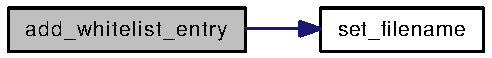
\includegraphics[width=186pt]{phonefirewall__administration_8c_eec16cb88eb546b1a2490e6716d75f8b_cgraph}
\end{center}
\end{figure}
\hypertarget{phonefirewall__administration_8c_f28c4b8fd3fdfe5e70df391cf40ca9f2}{
\index{phonefirewall\_\-administration.c@{phonefirewall\_\-administration.c}!check\_\-blacklist\_\-entry@{check\_\-blacklist\_\-entry}}
\index{check\_\-blacklist\_\-entry@{check\_\-blacklist\_\-entry}!phonefirewall_administration.c@{phonefirewall\_\-administration.c}}
\subsubsection{\setlength{\rightskip}{0pt plus 5cm}int check\_\-blacklist\_\-entry (int {\em country\_\-code}, int {\em area\_\-code}, unsigned long long {\em number}, int {\em priority})}}
\label{phonefirewall__administration_8c_f28c4b8fd3fdfe5e70df391cf40ca9f2}


Checks if a number is on the blacklist.

\begin{Desc}
\item[Parameters:]
\begin{description}
\item[{\em country\_\-code}]The country code (for example 39 for Italy, 43 for Austria, and so one) \item[{\em area\_\-code}]The area code which indicates your mobile operator. \item[{\em number}]The telephone number of the person (without country and area code. \item[{\em priority}]Gives the \hyperlink{structentry}{entry} a priority. 0 is standard. If the priority is higher the value will be also blocked/accepted if a higher priority is choosen.\par
 The value \char`\"{}PRIO\_\-ALL\char`\"{} stands for all priorities.\end{description}
\end{Desc}
\begin{Desc}
\item[Returns:]If the number was found 1, otherwise 0. \end{Desc}


Definition at line 215 of file phonefirewall\_\-administration.c.

References Entry::area\_\-code, Entry::country\_\-code, DB\_\-FILE, ERR\_\-FLAG, evaluate\_\-stmt(), INFO\_\-FLAG, MAX\_\-LINE\_\-LENGTH, Entry::number, Entry::priority, STMT\_\-SIZE, TB\_\-AREACODE, TB\_\-COUNTRYCODE, TB\_\-NUMBER, TB\_\-PRIORITY, and write\_\-logentry().

Here is the call graph for this function:\nopagebreak
\begin{figure}[H]
\begin{center}
\leavevmode
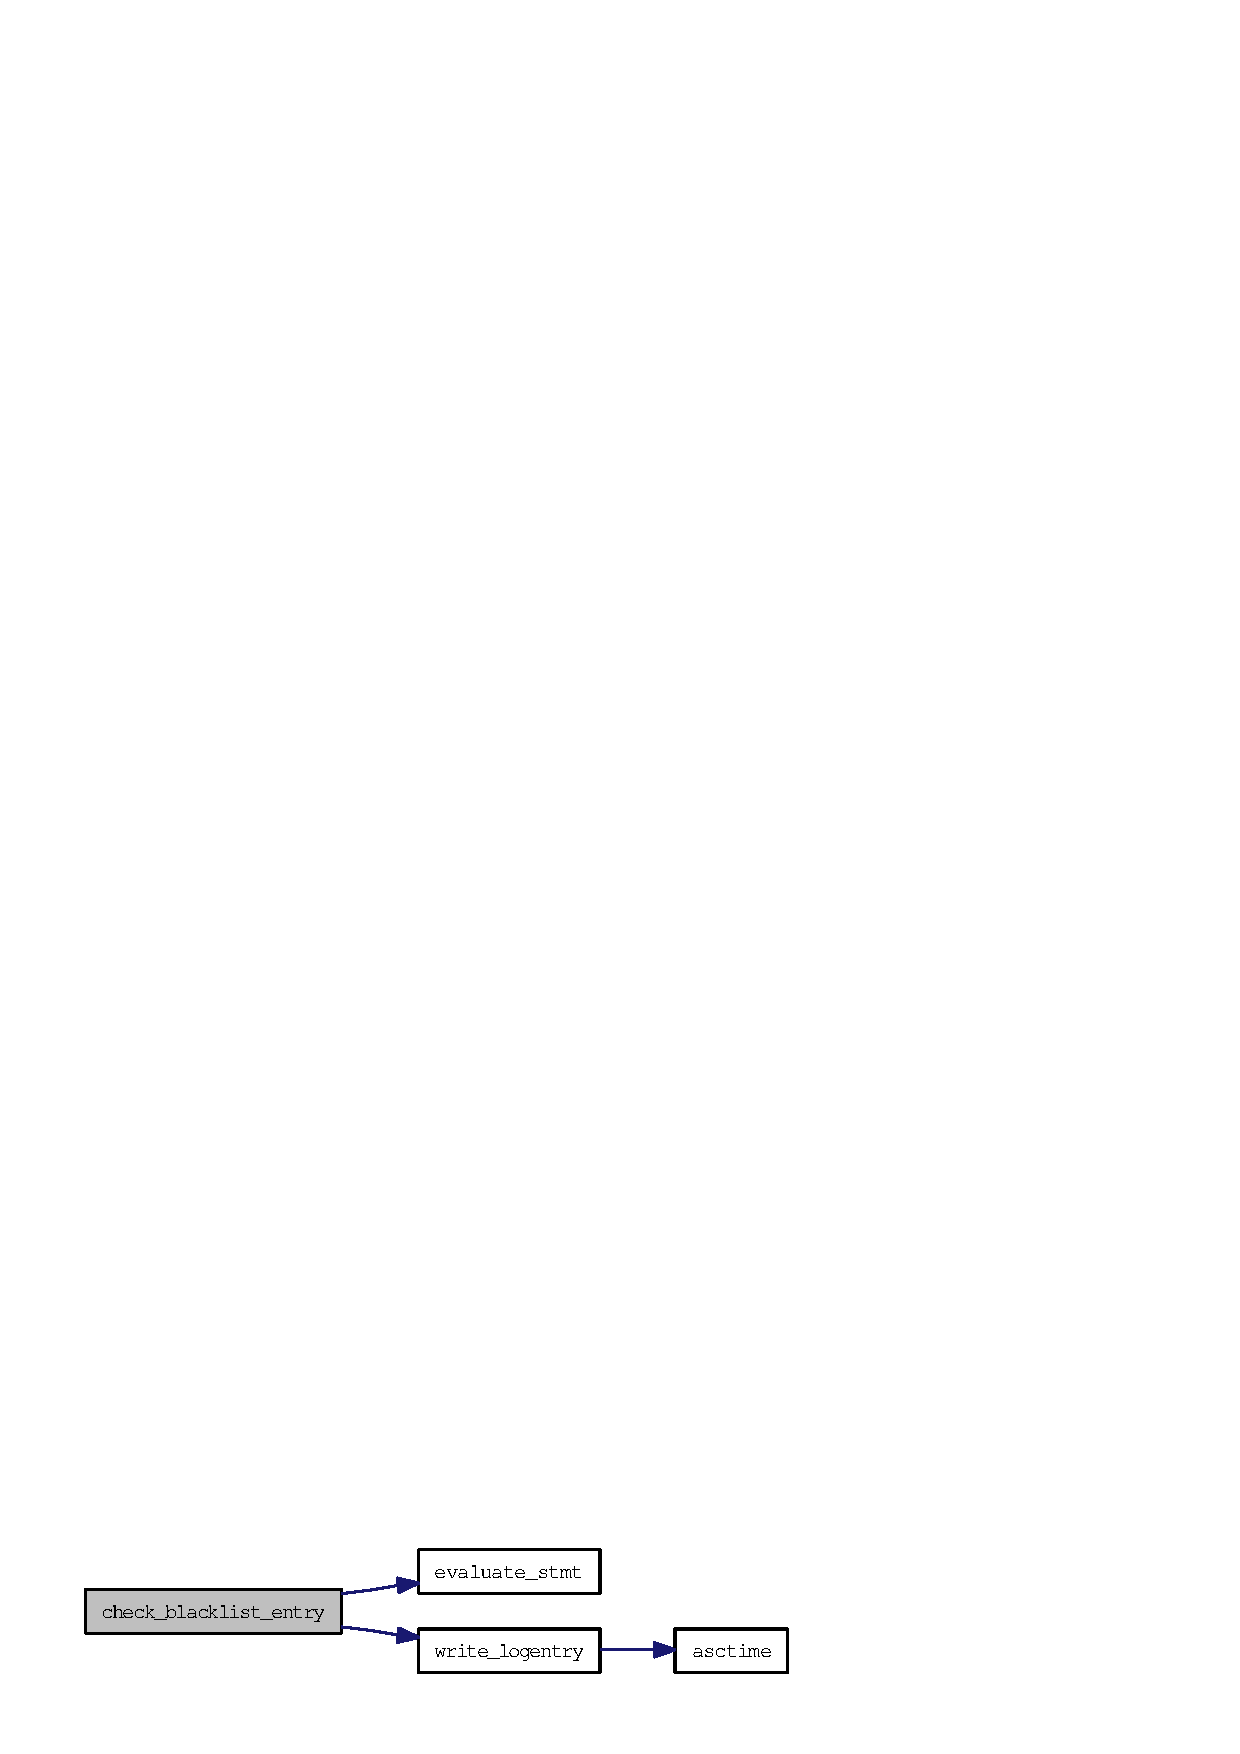
\includegraphics[width=191pt]{phonefirewall__administration_8c_f28c4b8fd3fdfe5e70df391cf40ca9f2_cgraph}
\end{center}
\end{figure}
\hypertarget{phonefirewall__administration_8c_f144fe0aa2eb227fe646da21048388a5}{
\index{phonefirewall\_\-administration.c@{phonefirewall\_\-administration.c}!check\_\-whitelist\_\-entry@{check\_\-whitelist\_\-entry}}
\index{check\_\-whitelist\_\-entry@{check\_\-whitelist\_\-entry}!phonefirewall_administration.c@{phonefirewall\_\-administration.c}}
\subsubsection{\setlength{\rightskip}{0pt plus 5cm}int check\_\-whitelist\_\-entry (int {\em country\_\-code}, int {\em area\_\-code}, unsigned long long {\em number}, int {\em priority})}}
\label{phonefirewall__administration_8c_f144fe0aa2eb227fe646da21048388a5}


Checks if a number is on the whitelist.

\begin{Desc}
\item[Parameters:]
\begin{description}
\item[{\em country\_\-code}]The country code (for example 39 for Italy, 43 for Austria, and so one) \item[{\em area\_\-code}]The area code which indicates your mobile operator. \item[{\em number}]The telephone number of the person (without country and area code. \item[{\em priority}]Gives the \hyperlink{structentry}{entry} a priority. 0 is standard. If the priority is higher the value will be also blocked/accepted if a higher priority is choosen.\par
 The value \char`\"{}PRIO\_\-ALL\char`\"{} stands for all priorities.\end{description}
\end{Desc}
\begin{Desc}
\item[Returns:]If the number was found 1, otherwise 0. \end{Desc}


Definition at line 270 of file phonefirewall\_\-administration.c.

References Entry::area\_\-code, Entry::country\_\-code, DB\_\-FILE, ERR\_\-FLAG, evaluate\_\-stmt(), INFO\_\-FLAG, MAX\_\-LINE\_\-LENGTH, Entry::number, Entry::priority, STMT\_\-SIZE, TB\_\-AREACODE, TB\_\-COUNTRYCODE, TB\_\-NUMBER, TB\_\-PRIORITY, and write\_\-logentry().

Here is the call graph for this function:\nopagebreak
\begin{figure}[H]
\begin{center}
\leavevmode
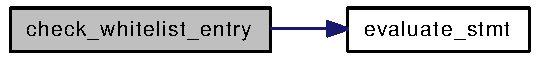
\includegraphics[width=192pt]{phonefirewall__administration_8c_f144fe0aa2eb227fe646da21048388a5_cgraph}
\end{center}
\end{figure}
\hypertarget{phonefirewall__administration_8c_f306b60195d745190ef3e30e7d0a107e}{
\index{phonefirewall\_\-administration.c@{phonefirewall\_\-administration.c}!evaluate\_\-stmt@{evaluate\_\-stmt}}
\index{evaluate\_\-stmt@{evaluate\_\-stmt}!phonefirewall_administration.c@{phonefirewall\_\-administration.c}}
\subsubsection{\setlength{\rightskip}{0pt plus 5cm}int evaluate\_\-stmt (sqlite3\_\-stmt $\ast$ {\em pp\_\-stmt}, struct {\bf Entry} $\ast$ {\em p\_\-entry})}}
\label{phonefirewall__administration_8c_f306b60195d745190ef3e30e7d0a107e}




Definition at line 28 of file phonefirewall\_\-administration.c.

References Entry::area\_\-code, Entry::country\_\-code, Entry::number, PRIO\_\-ALL, Entry::priority, TB\_\-AREACODE, TB\_\-COUNTRYCODE, TB\_\-NUMBER, and TB\_\-PRIORITY.

Referenced by check\_\-blacklist\_\-entry(), and check\_\-whitelist\_\-entry().

Here is the caller graph for this function:\nopagebreak
\begin{figure}[H]
\begin{center}
\leavevmode
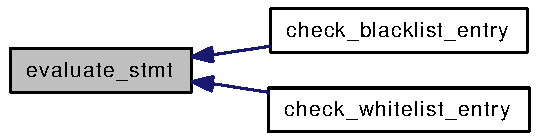
\includegraphics[width=147pt]{phonefirewall__administration_8c_f306b60195d745190ef3e30e7d0a107e_icgraph}
\end{center}
\end{figure}
\hypertarget{phonefirewall__administration_8c_4eee00c845ad4a60eaccef8c41151ea4}{
\index{phonefirewall\_\-administration.c@{phonefirewall\_\-administration.c}!rm\_\-blacklist\_\-entry@{rm\_\-blacklist\_\-entry}}
\index{rm\_\-blacklist\_\-entry@{rm\_\-blacklist\_\-entry}!phonefirewall_administration.c@{phonefirewall\_\-administration.c}}
\subsubsection{\setlength{\rightskip}{0pt plus 5cm}int rm\_\-blacklist\_\-entry (int {\em country\_\-code}, int {\em area\_\-code}, unsigned long long {\em number})}}
\label{phonefirewall__administration_8c_4eee00c845ad4a60eaccef8c41151ea4}


Removes a blocked number from the blacklist.

\begin{Desc}
\item[Parameters:]
\begin{description}
\item[{\em number}]The number which will be deleted.\end{description}
\end{Desc}
\begin{Desc}
\item[Returns:]If all goes right 0, otherwise an error code. \end{Desc}


Definition at line 146 of file phonefirewall\_\-administration.c.

References DB\_\-FILE, ERR\_\-FLAG, MAX\_\-LINE\_\-LENGTH, STMT\_\-SIZE, TB\_\-AREACODE, TB\_\-COUNTRYCODE, TB\_\-NUMBER, and write\_\-logentry().

Here is the call graph for this function:\nopagebreak
\begin{figure}[H]
\begin{center}
\leavevmode
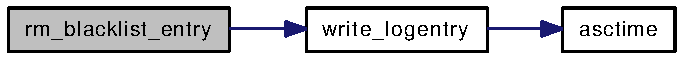
\includegraphics[width=182pt]{phonefirewall__administration_8c_4eee00c845ad4a60eaccef8c41151ea4_cgraph}
\end{center}
\end{figure}
\hypertarget{phonefirewall__administration_8c_307d220ee8e63926af279460532787ff}{
\index{phonefirewall\_\-administration.c@{phonefirewall\_\-administration.c}!rm\_\-whitelist\_\-entry@{rm\_\-whitelist\_\-entry}}
\index{rm\_\-whitelist\_\-entry@{rm\_\-whitelist\_\-entry}!phonefirewall_administration.c@{phonefirewall\_\-administration.c}}
\subsubsection{\setlength{\rightskip}{0pt plus 5cm}int rm\_\-whitelist\_\-entry (int {\em country\_\-code}, int {\em area\_\-code}, unsigned long long {\em number})}}
\label{phonefirewall__administration_8c_307d220ee8e63926af279460532787ff}


Removes a accepted number from the whitelist.

\begin{Desc}
\item[Parameters:]
\begin{description}
\item[{\em number}]The number which will be deleted.\end{description}
\end{Desc}
\begin{Desc}
\item[Returns:]If all goes right 0, otherwise an error code. \end{Desc}


Definition at line 180 of file phonefirewall\_\-administration.c.

References DB\_\-FILE, ERR\_\-FLAG, MAX\_\-LINE\_\-LENGTH, STMT\_\-SIZE, TB\_\-AREACODE, TB\_\-COUNTRYCODE, TB\_\-NUMBER, and write\_\-logentry().

Here is the call graph for this function:\nopagebreak
\begin{figure}[H]
\begin{center}
\leavevmode
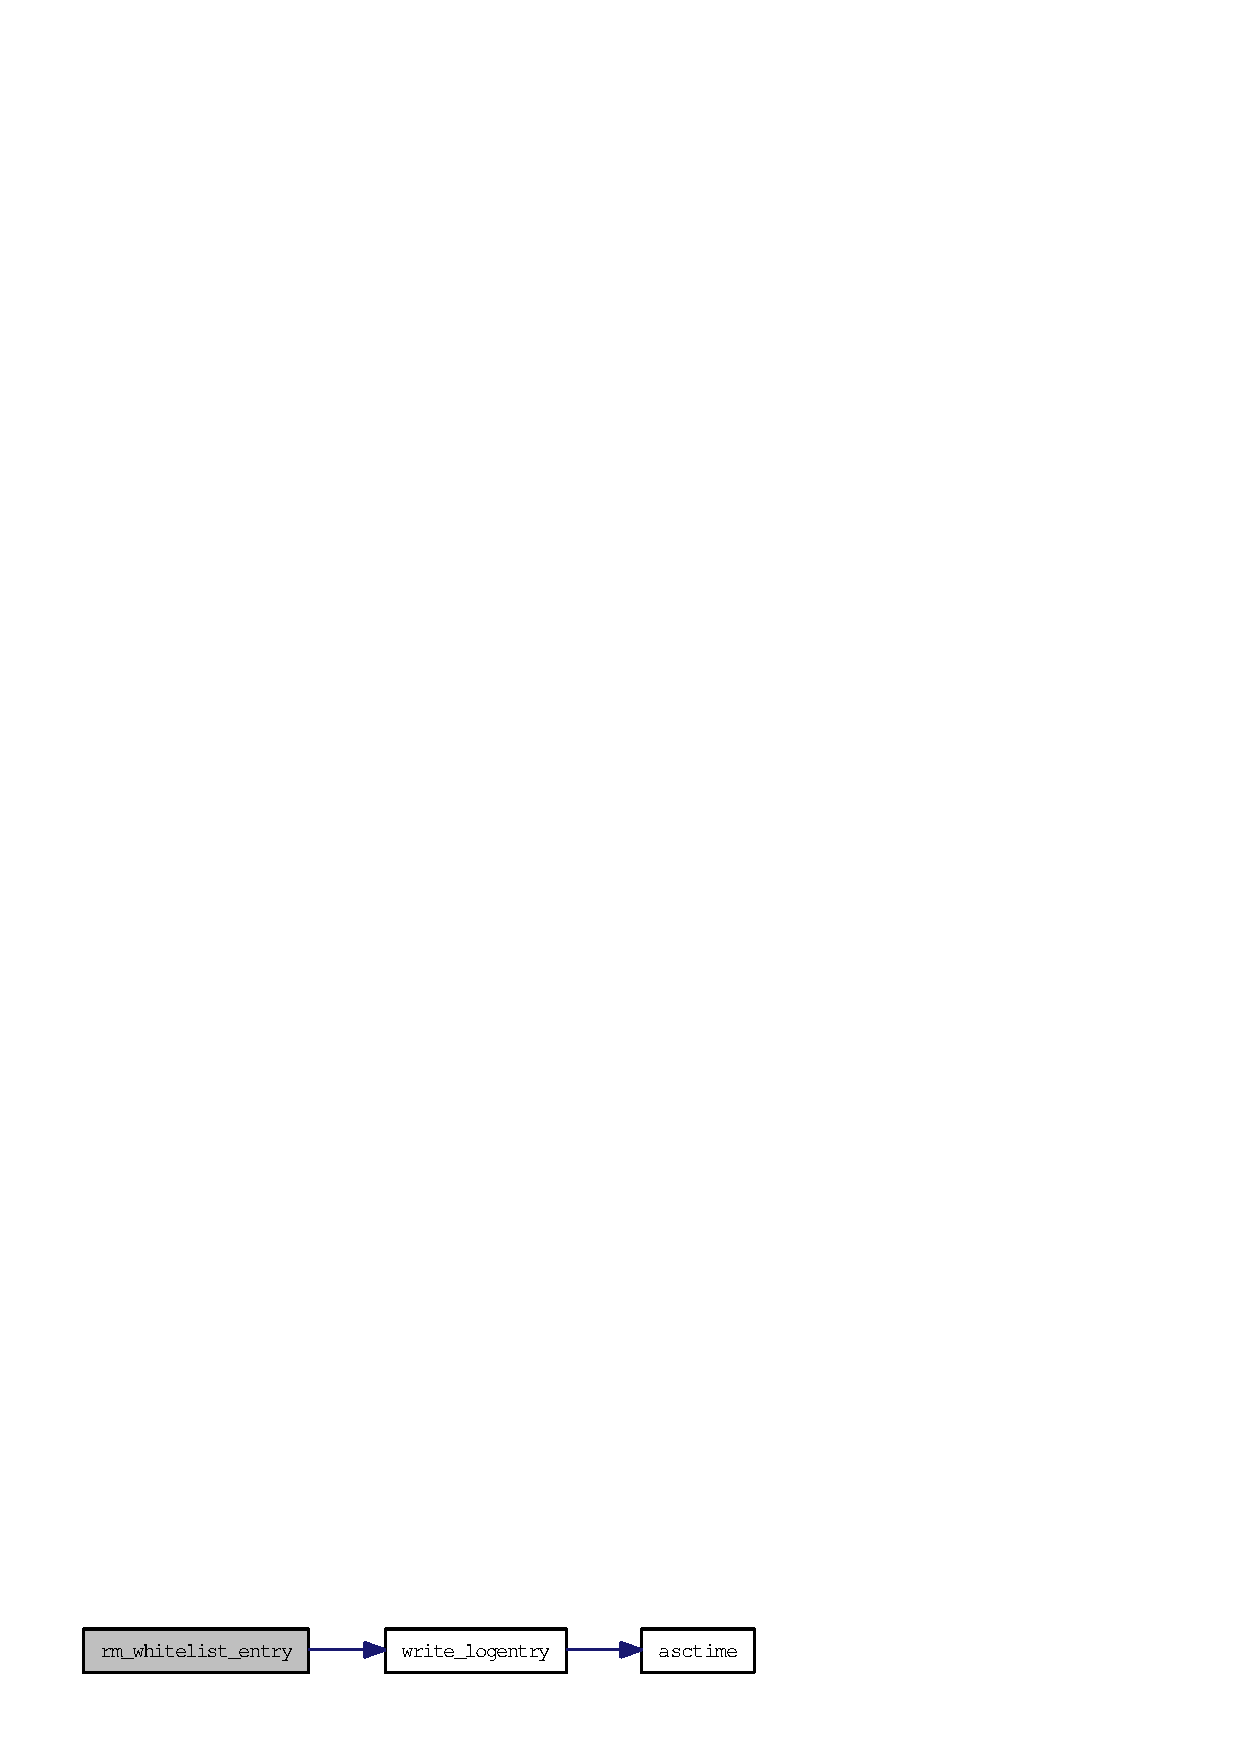
\includegraphics[width=183pt]{phonefirewall__administration_8c_307d220ee8e63926af279460532787ff_cgraph}
\end{center}
\end{figure}
